\documentclass{beamer} % [handout] para imprimir eliminando transiciones

%\usefonttheme[onlymath]{serif}
%\usepackage{fontspec}
%\defaultfontfeatures{Mapping=tex-text}
%\setsansfont[Ligatures={Common}]{Futura}
%\setmonofont[Scale=0.8]{Monaco} 

\usepackage{beamerthemesplit}
\usepackage[utf8]{inputenc}
\usepackage[spanish]{babel}
\mode<presentation>
\usetheme{default}
\usecolortheme{dolphin}
\usepackage{alltt}    % \begin{alltt}
\usepackage{amssymb}  % mathematical symbols
\usepackage{comment}
\usepackage{multicol} % \multicols
\usepackage{multirow} % \multirows
\usepackage{tabto}    % \tabto
\usepackage{verbatim} % comentarios

\title{Estructuras de datos}   %[titulo corto]
\author{Fabián Riquelme Csori} %[nombre corto]
\date{2017}                    %[fecha corta]
\institute{Universidad de Valparaíso}                 %[instituto corto]

\newcommand{\HRule}{\rule{\linewidth}{0.2mm}\\[1ex]}
\newcommand{\blue}[1]{\textcolor{blue}{#1}}
\newcommand{\red}[1]{\textcolor{red}{#1}}
\newcommand{\redb}[1]{{\color{red!70!black}{#1}}}
\newcommand{\green}[1]{{\color{green!70!black}{#1}}}
\newcommand{\gray}[1]{{\color{gray!50!white}{#1}}}
\newcommand{\textgreek}[1]{\begingroup\fontencoding{LGR}\selectfont#1\endgroup}
% \alert{texto destacado en rojo}
% \color{green} Color en verde
% \structure{texto en lila}

\begin{document}


%\begin{frame}%[plain]
%  \titlepage
%\end{frame}
%
% [opciones]:
% plain: oculta barra de navegacion, deja + espacio para contenido
% fragile: usar comandos como verbatim
% b,c,t: alineacion vertical
% label=nombre_etiqueta
% allowframebreaks: divide contenido en varios frames si es demasiado largo
% shrink: para escribir mucho texto en una transparencia, reduciendo tamano de fuente

%%%%%%%%%% PORTADA %%%%%%%%%%
\begin{frame}[plain]
  \begin{figure}[h]
    \begin{minipage}{0.3\textwidth}
    
\includegraphics[width=.9\textwidth]{./image/logo-UV.png}
    \end{minipage}
    \begin{minipage}{0.65\textwidth}
     $~$\\[3.6ex]
     \footnotesize{Escuela de Ingeniería Civil Informática}\\
     \footnotesize{Facultad de Ingeniería}
    \end{minipage}
  \end{figure}
  \begin{center}
    \vspace{1ex}
    \HRule
    \Large{Estructuras de datos}\\{\small Capítulo VI: Grafos}\\[-1ex]
    \HRule\vspace{1ex}
    \large{Fabián Riquelme Csori}\\[.5ex]\footnotesize{fabian.riquelme@uv.cl}\\[6ex] {\tiny 2017-II}\\[6ex]
  \end{center}
\end{frame}

%%%%%%%%%% INDEX %%%%%%%%%%
\begin{frame}
 \frametitle{Index}
 \scriptsize 			% reducir tamano de letra
 \tableofcontents		%[pausesections]
\end{frame}

%%%%%%%%%%% ACTUAL INDEX %%%%%%%%%%
%\AtBeginSection[] %generar indice automaticamente
%{
%\begin{frame}<beamer>%[plain]
% \frametitle{Index}
% \framesubtitle{subtitulo}
% \scriptsize
% \tableofcontents[currentsection, currentsubsection]
%\end{frame}
%}

%==============================
\section{Grafos}

%-----------------------
\subsection{Fundamentos}

\begin{frame}{Teoría de grafos}
    \begin{itemize}
        \item<1-> Un \blue{grafo} es un par ordenado $G=(V,E)$ donde
        \begin{itemize}
            \item $V$ es un conjunto de nodos o vértices.
            \item $E$ es un conjunto de aristas.
        \end{itemize}
        \item<2-> Decimos que $|E|=m$ y el \blue{orden} de $G$ es $|V|=n$.
        \item<3-> Si $G$ es \blue{dirigido} y $a\in V$, entonces: 
        \begin{itemize}
            \item $\delta^-(a)=|\{x\in V\mid (x,a)\in E\}|$ es el \blue{grado de entrada} de $a$.
            \item $\delta^+(a)=|\{x\in V\mid (a,x)\in E\}|$ es el \blue{grado de salida} de $a$.
        \end{itemize}
        \item<3-> Si $G$ es \blue{no-dirigido} y $a\in V$, entonces:
        \begin{itemize}
            \item $\delta(a)=|\{x\in V\mid \{a,x\}\in E\}|$ es el \blue{grado} de $a$.
        \end{itemize}
        \item<4-> Los grafos representan \blue{relaciones}.
        \begin{itemize}
            \item ¿Cómo es un $G$ reflexivo, simétrico, antisimétrico, transitivo?
        \end{itemize}
        \item<5-> Los grafos pueden ser además \blue{etiquetados} ({\em labeled})\\ y \blue{con pesos} ({\em weighted}).
    \end{itemize}
\end{frame}

\begin{frame}{Aplicaciones}
    \begin{minipage}{0.55\textwidth}
      {\small
      \begin{itemize}
        \item Redes de computadores
        \item Telecomunicaciones
        \item Análisis de redes sociales
        \item Computación gráfica
        \item Representación del conocimiento
        \item Teoría de autómatas
        \item Teoría de compiladores
        \item Circuitos digitales
        \item Bioinformática
        \item Machine learning
        \item etc. etc. etc.
      \end{itemize}}
    \end{minipage}
    \begin{minipage}{0.4\textwidth}
      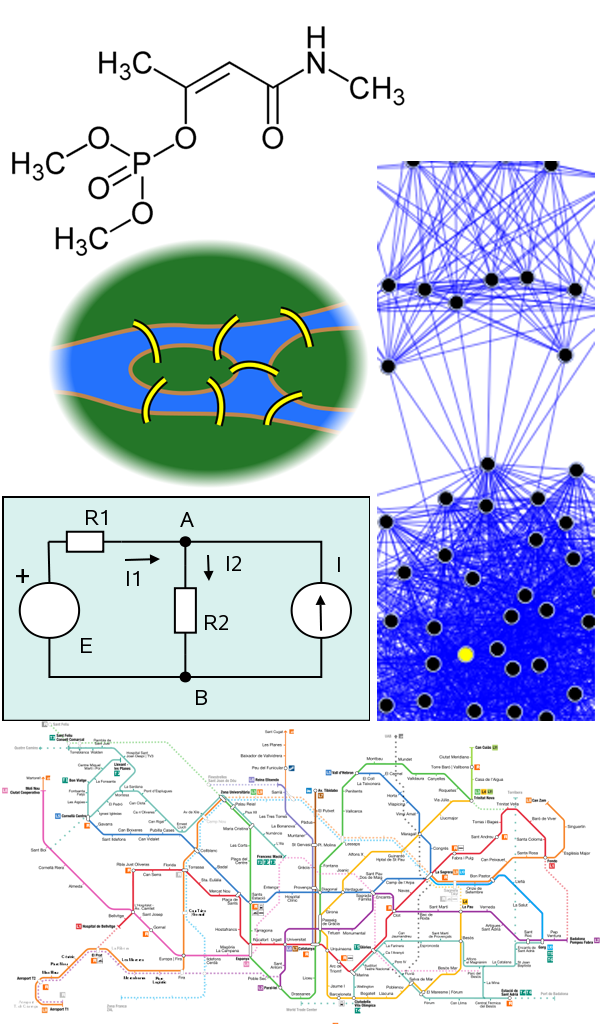
\includegraphics[width=\textwidth]{./image/cap6/grafos-aplicaciones.png}
    \end{minipage}
\end{frame}

%-----------------------
\subsection{Grafos como TDA}

\begin{frame}{Grafos como TDA}
    \scriptsize{
    \begin{tabular}{lp{60ex}}\hline\\[-1ex]
      {\bf\normalsize grafo} & Relaciones binarias entre vértices.\\[2ex]
      {\bf\small operations}  & \\[1.5ex]
      isAdjacent(G,x,y) & Is there an edge from the vertex x to the vertex y?\\
      neighbors(G,x)    & lists all vertices y s.t. $\exists$ an edge from vertex x to vertex y.\\
      add\_vertex(G,x)   & adds the vertex x, if it is not there.\\
      remove\_vertex(G,x)& removes the vertex x, if it is there.\\
      add\_edge(G,x,y)   & adds the edge (x,y) if it is not there.\\
      remove\_edge(G,x,y)& removes the edge (x,y) if it is there.\\[1.5ex]
      get\_vertex\_value(G,x) & returns the value (label) associated with vertex x.\\
      set\_vertex\_value(G,x,v) & sets the value (label) associated with vertex x to v.\\[1.5ex]
      get\_edge\_value(G,x,y) & returns the value (weight) associated with edge (x,y).\\
      set\_edge\_value(G,x,y,v) & sets the value (weight) associated with edge (x,y) to v.\\[1.5ex]\hline
    \end{tabular}}
\end{frame}

%-----------------------
\subsection{Representación de grafos}

\begin{frame}{Representación de grafos}
    \begin{itemize}
        \item<1-> Los grafos se pueden representar e implementar mediante diversas estructuras de datos.
        \item<1-> Una manera usual es como \blue{lista de aristas} ``{\scriptsize\texttt{nodo\_ini nodo\_fin}}''.
        \begin{itemize}
            \item Se favorece simplicidad de almacenamiento en archivos CSV.
            \item Formato adaptable a pesos de aristas y otros datos adicionales.
        \end{itemize}
        \item<2-> Tres maneras usuales más pensadas en la manipulación que solo en el almacenamiento:
        \begin{itemize}
            \item \blue{Lista de adyacencia}
            \item \blue{Matriz de adyacencia}
            \item \blue{Matriz de incidencia}
        \end{itemize}
    \end{itemize}
\end{frame}

\begin{frame}{Lista de adyacencia}
    \begin{center}
      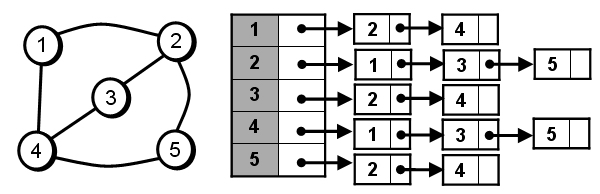
\includegraphics[width=\textwidth]{./image/cap6/lista-adyacencia.jpg}
    \end{center}
    \begin{itemize}
        \item Cada nodo de la lista puede almacenar información adicional.
        \item Representación útil para \blue{grafos dispersos} ({\em sparse graphs}),\\
        i.e., aquellos con $|E|=O(|V|)$.
    \end{itemize}
\end{frame}

\begin{frame}{Matriz de adyacencia}
    \begin{center}
      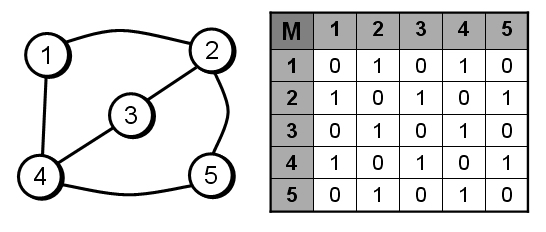
\includegraphics[width=.8\textwidth]{./image/cap6/matriz-adyacencia.jpg}
    \end{center}
    \begin{itemize}
        \item Fácil incluir pesos en aristas.
        \item Representación útil para \blue{grafos densos} ({\em dense graphs}),\\
        i.e., aquellos con $|E|=O(|V|^2)$.
    \end{itemize}
\end{frame}


\begin{frame}{Matriz de incidencia}
    \begin{center}
      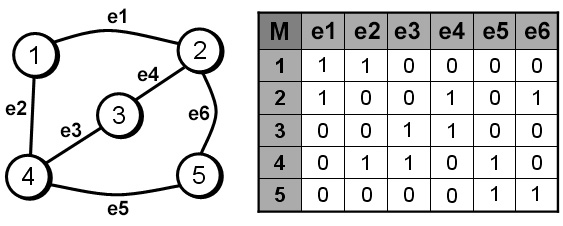
\includegraphics[width=.8\textwidth]{./image/cap6/matriz-incidencia.jpg}
    \end{center}
    \begin{itemize}
        \item En general se utiliza mucho menos.
        \item Mejor que matriz de adyacencia para ciertas operaciones cuando $|V|\cdot|E|<|V|^2$, si bien en tales casos conviene más la lista de adyacencia.
    \end{itemize}
\end{frame}

\begin{frame}{Comparaciones}
    \begin{center}
      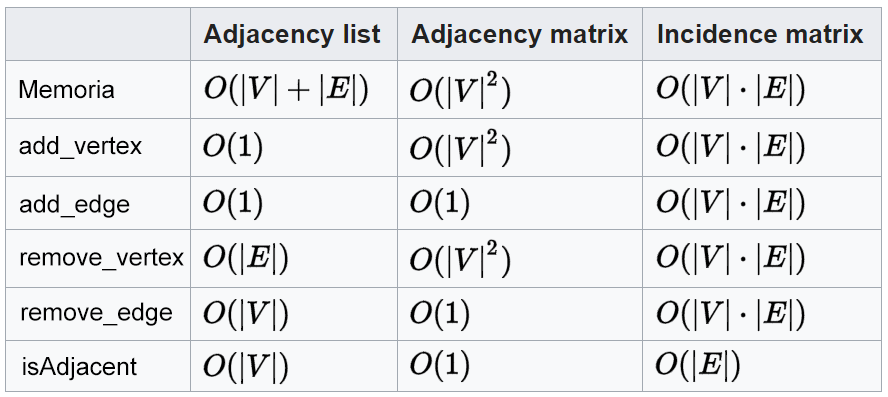
\includegraphics[width=\textwidth]{./image/cap6/represent-complexity.png}
    \end{center}
    \begin{itemize}
        \item ¿Qué pasa con la memoria en listas de adyacencia:
        \begin{itemize}
            \item ...si el grafo es disperso? \uncover<2->{$O(|V|)$.}
            \item ...si el grafo es denso? \uncover<3->{$O(|V|^2)$.}
        \end{itemize}
    \end{itemize}
\end{frame}

%==============================
\section{Problemas de grafos}

%-----------------------
\subsection{Problemas de cobertura}

\begin{frame}{Cobertura de vértices (vertex cover)}
    \begin{itemize}
        \item<1-> Una \blue{cobertura de vértices} de un grafo $G=(V,E)$ es un conjunto de vértices $V'\subseteq V$ tal que cada arista de $G$ es incidente a al menos un vértice de $V'$.
        \uncover<2->{
        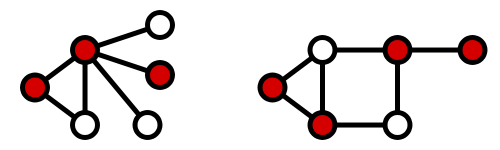
\includegraphics[width=.6\textwidth]{./image/cap6/vertex-cover.png}}
        \item<3-> Una \blue{cobertura de vértices mínima} es una cobertura de vértices $V'$ tal que quitando un vértice de $V'$ se pierde la cobertura.
        \uncover<4->{
        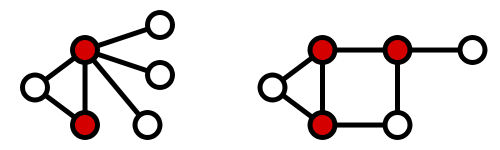
\includegraphics[width=.6\textwidth]{./image/cap6/min-vertex-cover.png}}
    \end{itemize}
\end{frame}

\begin{frame}{Cobertura de aristas (edge cover)}
    \begin{itemize}
        \item<1-> Una \blue{cobertura de aristas} de un grafo $G=(V,E)$ es un conjunto de aristas $E'\subseteq E$ tal que cada vértice de $G$ es incidente en al menos una arista de $E'$.
        \uncover<2->{
        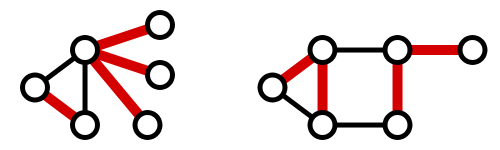
\includegraphics[width=.6\textwidth]{./image/cap6/edge-cover.png}}
        \item<3-> Una \blue{cobertura de aristas mínima} es una cobertura de aristas $E'$ tal que quitando una arista de $E'$ se pierde la cobertura.
        \uncover<4->{
        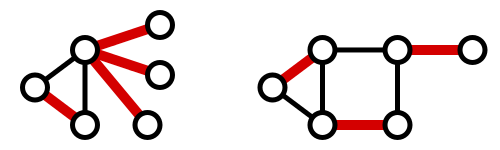
\includegraphics[width=.6\textwidth]{./image/cap6/min-edge-cover.png}}
    \end{itemize}
\end{frame}

\begin{frame}{Ejercicios}
    \begin{itemize}
        \item Implemente un generador de \blue{grafos aleatorios}, que recibe como input $|V|=n$ y por cada par de vértices $\{a,b\}\subseteq V$ crea una arista $(a,b)\in E$ con probabilidad $p=0.5$.
        \item Utilice como estructura de datos para almacenar el grafo:
        \begin{enumerate}
            \item Una matriz de adyacencia.
            \item Una lista de adyacencia.
        \end{enumerate}
        \item Implemente una función que reciba como entrada un conjunto $V'\subseteq V$ y como salida responda {\em Sí} si $V'$ es una cobertura de vértices, y {\em No} en caso contrario.
        \item Repita el ejercicio anterior para el caso de cobertura mínima, y para las respectivas coberturas de aristas.
        \item Investigue lo que es un \blue{grafo bipartito} y repita todos los ejercicios anteriores para esta familia de grafos. Note que los algoritmos de cobertura deberían ser más eficientes.
    \end{itemize}
\end{frame}

%-----------------------
\subsection{Problema del camino más corto}

\begin{frame}{Caminos}
    \begin{itemize}
        \item<1-> Dado un grafo, un \blue{camino} es una secuencia de vértices conectados por aristas.
        \begin{itemize}
            \item<2-> Un \blue{camino hamiltoniano} es uno que visita cada vértice del grafo una única vez.
            \item<3-> Un \blue{camino euleriano} es uno que visita cada arista del grafo una única vez.
        \end{itemize}
        \item<4-> Dos vértices están \blue{conectados} si existe un camino entre ellos.
        \begin{center}
        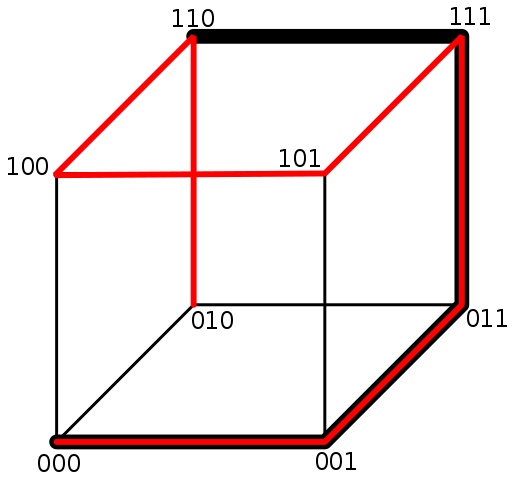
\includegraphics[width=.3\textwidth]{./image/cap6/camino.png}
        \end{center}
    \end{itemize}
\end{frame}

\begin{frame}{Grafos y componentes conexos}
    \begin{itemize}
        \item<1-> Un \blue{grafo conexo} es un grafo donde todo par de vértices está conectado mediante al menos un camino.
        \item<2-> Una \blue{componente conexa} es un \blue{subgrafo} que conforma un grafo conexo.
        \uncover<3->{
        \begin{flushright}
          ¿Cómo son los caminos de un grafo bipartito?
        \end{flushright}}
    \end{itemize}
\end{frame}

\begin{frame}{Problema del camino más corto}
    \begin{itemize}
        \item<1-> Un \blue{camino más corto} de un vértice a otro es uno que pasa por el menor número posible de vértices intermedios.
        \item<2-> El \blue{problema del camino más corto} consiste en dados dos vértices, encontrar el camino más corto entre ellos.
        \begin{itemize}
            \item<3-> Existen versiones para grafos dirigidos, no-dirigidos, y ponderados o con pesos.
        \end{itemize}
        \item<4-> A diferencia de los problemas de cobertura, este problema puede resolverse en tiempo polinomial.
        \begin{itemize}
          \item \blue{Algoritmo de Dijkstra}
          \item \blue{Algoritmo de Bellman-Ford}
          \item \blue{Algoritmo de Búsqueda $A^{\star}$}
          \item \blue{Algoritmo de Floyd-Warshall}
          \item \blue{Algoritmo de Johnson}
        \end{itemize}
    \end{itemize}
\end{frame}

\begin{frame}{Algoritmo de Dijkstra}
    \begin{itemize}
        \item Calcula todos los caminos más cortos desde un vértice a todos los demás del grafo.
    \end{itemize}
    \begin{center}
    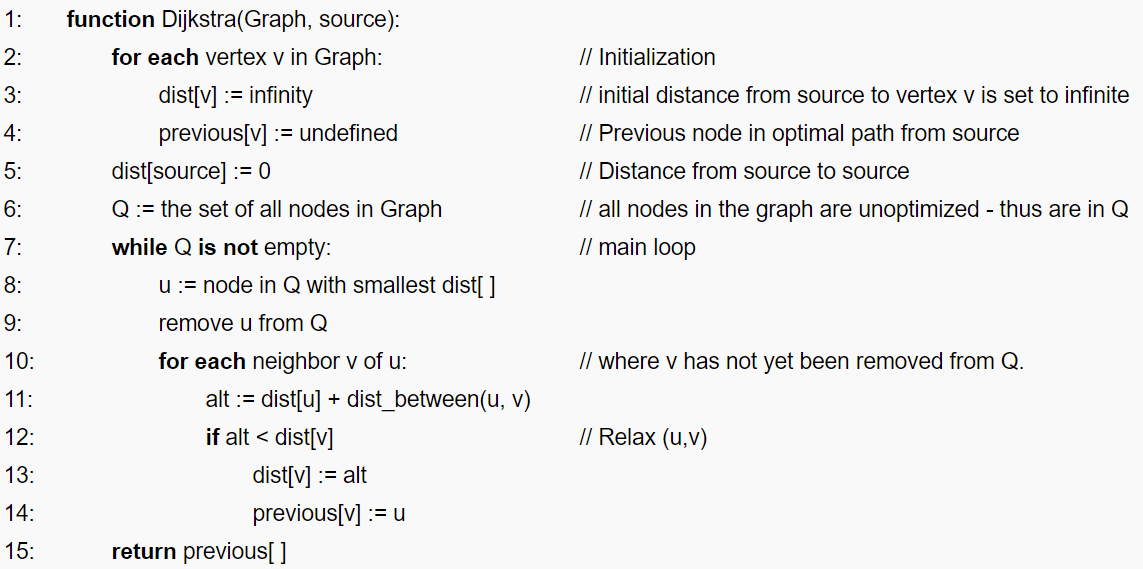
\includegraphics[width=\textwidth]{./image/cap6/dijkstra.png}
    \end{center}
\end{frame}

\begin{frame}{Ejercicio}
  \begin{enumerate}
    \item Ingrese a los contenidos del curso en el Aula Virtual y descargue el archivo \blue{\texttt{grafo-cap6.csv}}.
    \item A mano, utilice el algoritmo de Dijkstra para encontrar todos los caminos más cortos desde el vértice 1 al resto de los vértices del grafo.
    \item Implemente un programa que almacene este grafo en una matriz de adyacencia.
    \item Implemente el algoritmo de Dijkstra para validar sus resultados obtenidos en el punto 2.
  \end{enumerate}
  \begin{flushright}
    \blue{bonus +1} (en clases)
  \end{flushright}
\end{frame}

%------------------------------

\begin{frame}
 \begin{block}{Bibliografía recomendada}
  \begin{itemize}
    \item Weiss, M., Estructura de datos y algoritmos,\\ Addison-Wesley, 1995.
    \item Aho, Hopcroft y Ullman, Estructuras de datos y algoritmos, Addison-Wesley, 1988.
  \end{itemize}
 \end{block}
 \begin{block}{Recursos}
  \begin{itemize}
    \item Wikimedia Commons.
  \end{itemize}
 \end{block}
\end{frame}

\end{document}
